This section presents our complete method for accurate crowd counting on railway platforms. We propose a detect–track–count pipeline that combines YOLOv11m head detection, EfficientNet-B0-based ReID feature extraction, and a physics-constrained 3D Kalman filter for robust multi-object tracking. Our key innovation is the Phys-5D physics-constrained tracker that leverages camera geometry and scene priors to stabilize identity consistency and achieve superior counting accuracy.

\subsection{System Architecture}

We tackle platform crowd counting with a detect–track–count pipeline tailored to station-arrival videos with dense occlusions and strong perspective effects. The system integrates YOLOv11-based object detection, EfficientNet-B0 ReID feature extraction, and a 3D physical Kalman filter for robust pedestrian tracking.

\begin{figure}[htbp]
    \centering
    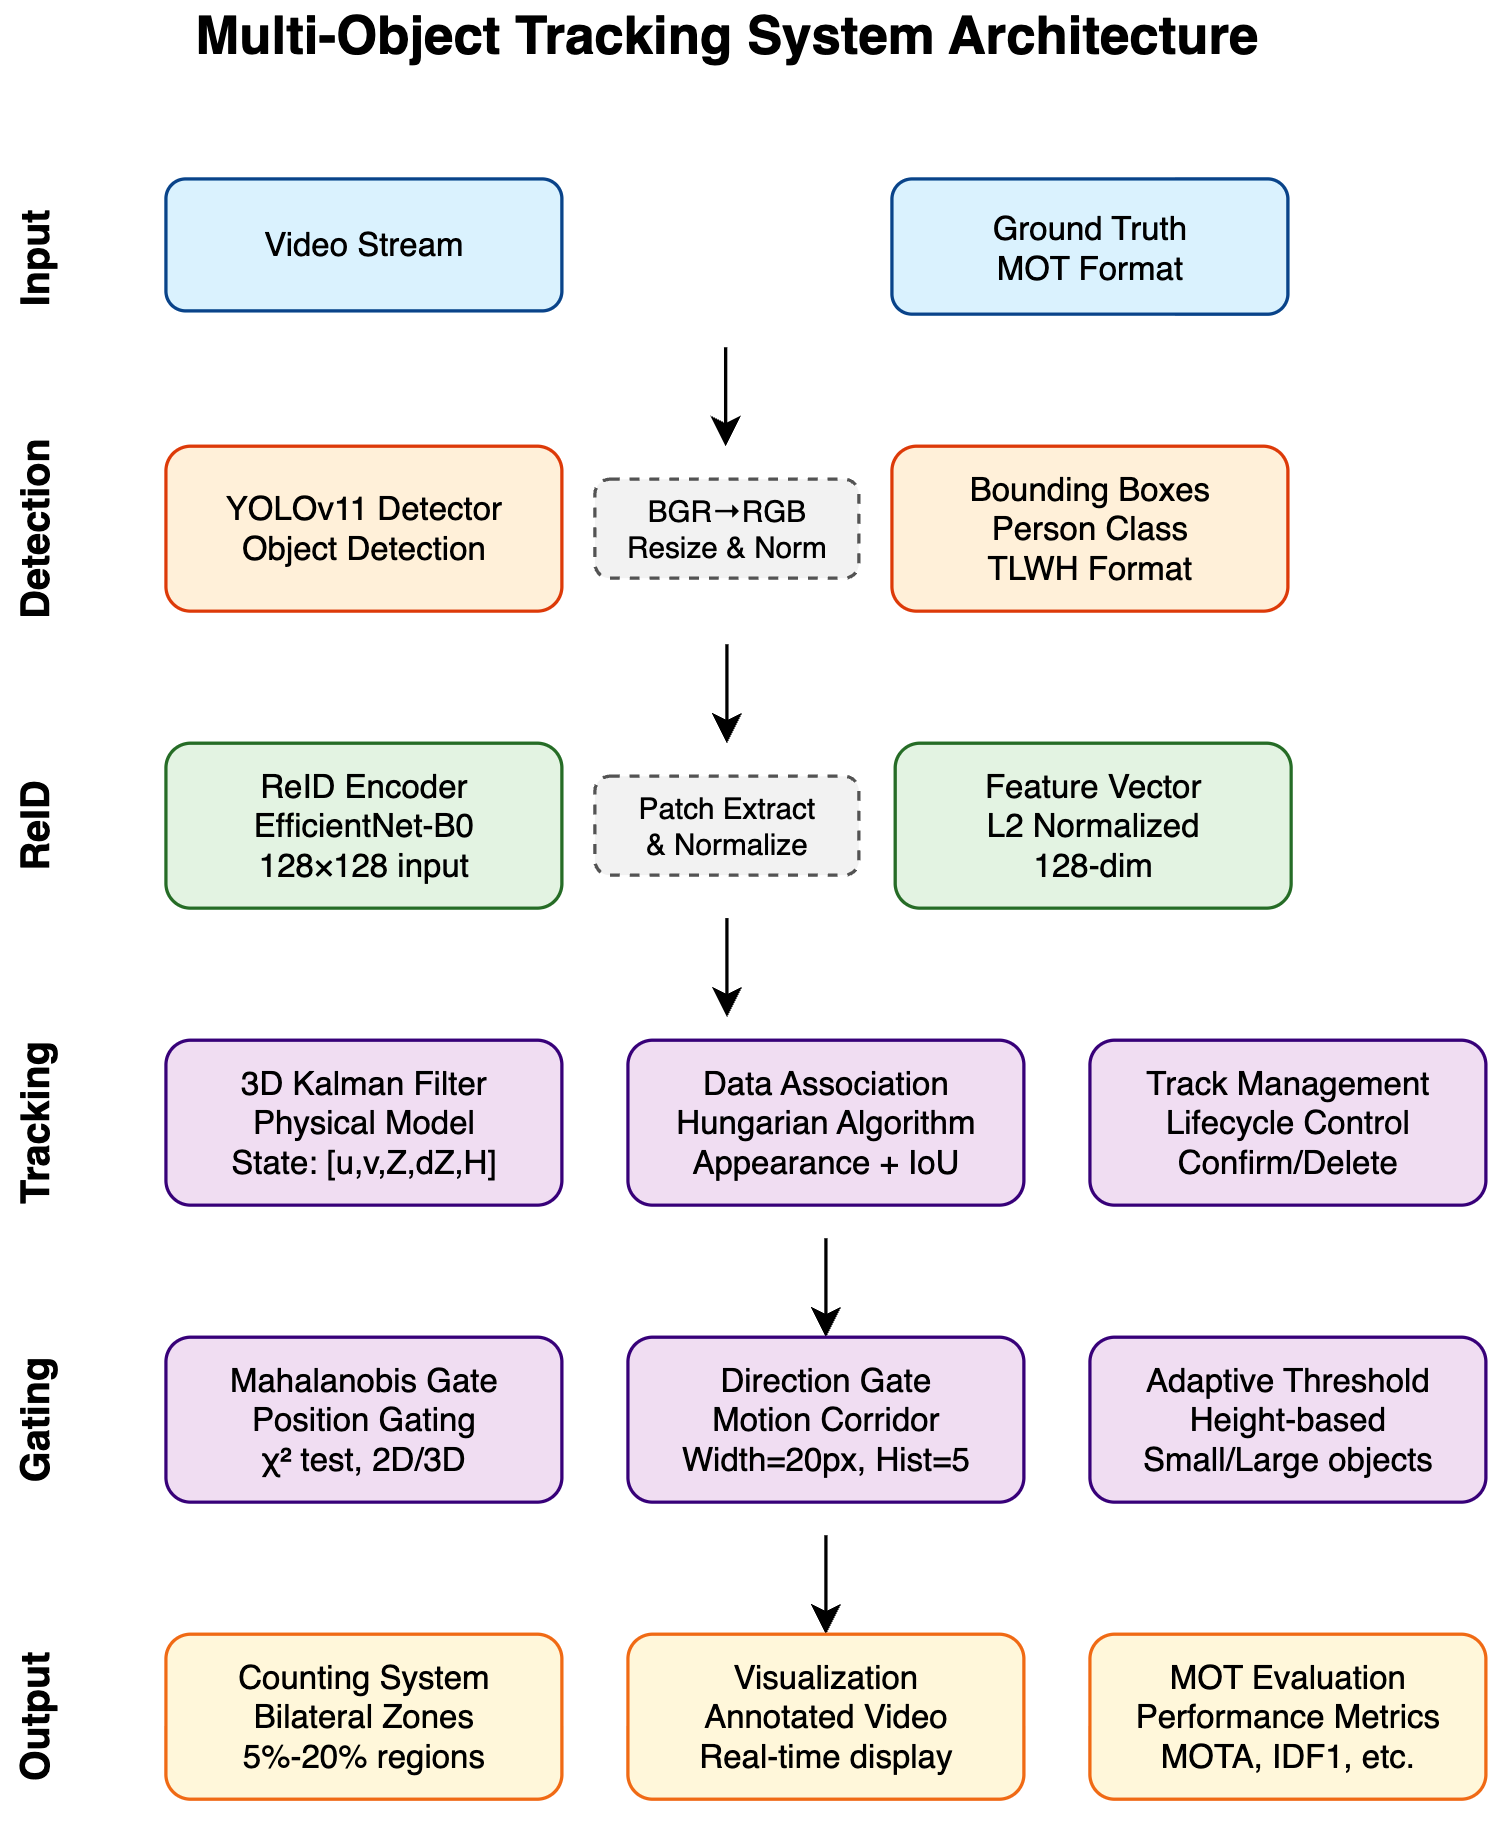
\includegraphics[width=0.49\textwidth]{pictures/OurMulti-ObjectTrackingSystemArchitecture.png}
    \caption{Overall Multi-object Tracking System Architecture. The system integrates YOLOv11-based object detection, EfficientNet-B0 ReID feature extraction, and a 3D physical Kalman filter for robust pedestrian tracking. The pipeline consists of five modules: (1) Input, which includes video streams and ground-truth annotations in MOT format; (2) Detection, where YOLOv11 detects pedestrian bounding boxes (TLWH format); (3) ReID, which extracts 128-dimensional L2-normalized feature vectors using an EfficientNet-B0 encoder; (4) Tracking and Gating, which performs data association via a Hungarian algorithm combining appearance and IoU metrics, managed by a 3D Kalman filter with state variables [u, v, z, dZ, H] and multiple gating strategies including Mahalanobis distance, directional motion corridors, and adaptive thresholds; and (5) Output, which provides bilateral-zone counting, annotated visualization, and MOTChallenge performance evaluation (MOTA, IDF1, etc.). This modular architecture ensures accurate, stable, and interpretable tracking across video sequences.}
    \label{fig:OurMOTSystemArchitecture}
\end{figure}


\subsection{Dataset and Preprocessing}

We constructed a comprehensive multi-modal dataset ecosystem for our experiments. The dataset includes:

\textbf{Training Data:} We use CrowdHuman dataset \cite{shao2018crowdhuman} (15,000 training images, 4,370 validation images) for pre-training, followed by fine-tuning on 2,000 annotated railway platform images from three sources: Open Sensor Data for Rail 2023 \cite{OpenSensorDataforRail2023} (20 images, 180 instances), RailEye3D Dataset \cite{RailEye3D_Dataset} (320 images, 1,221 instances), and our RailwayPlatformCrowd Dataset (1,660 images, 5,831 instances).

\textbf{Evaluation Dataset:} For comprehensive evaluation, we constructed the MOT-RailwayPlatformCrowdHead (MOT-RPCH) dataset containing 27 video sequences with 24,788 frames, 89,087 bounding boxes, and 885 unique human head identities. We select a representative subset of 20 video sequences for evaluation, spanning multiple resolutions (1536×864 to 2304×1296), frame rates (25, 29.97, 59.94 FPS), and target scales, totaling 18,548 frames, 647 identities, and 73,799 bounding boxes.

\subsection{YOLO and DeepSORT: Background and Limitations}

\textbf{YOLO (You Only Look Once):} YOLO \cite{redmon2016you} revolutionized object detection by formulating detection as a regression problem, enabling real-time performance through single-pass inference. However, in crowded railway platform scenarios, YOLO faces significant challenges: (1) severe occlusions between pedestrians degrade detection accuracy, (2) small head targets are difficult to localize consistently, and (3) perspective effects cause scale variations that confuse standard detection approaches.

\textbf{DeepSORT:} DeepSORT \cite{211} extends SORT by incorporating deep appearance embeddings with motion information through a Kalman filter. While effective for general tracking scenarios, DeepSORT has inherent limitations in railway platform contexts: (1) the standard 8D constant-velocity model assumes linear motion, which fails under train deceleration, (2) 2D image-plane tracking cannot leverage 3D scene geometry, and (3) identity switches increase dramatically under dense occlusions and perspective effects.

These limitations motivate our physics-constrained 3D tracking approach that explicitly models train deceleration and leverages camera geometry for improved accuracy.

\subsection{YOLOv11 Head Detection}

We adopt YOLOv11m for head detection to reduce occlusion-induced misses and stabilize localization for small targets. Our approach uses two-stage transfer learning:

\textbf{Stage 1:} Pre-training on CrowdHuman dataset achieves mAP50=79.4\% and mAP50–95=54.7\%.

\textbf{Stage 2:} Fine-tuning with backbone=10 frozen on railway platform head images achieves mAP50=98.0\% (+18.6 points) and mAP50–95=81.6\% (+26.9 points).

The detector uses SGD optimizer (lr=0.01, momentum=0.937, weight decay=0.0005), cosine annealing scheduler, and mixed precision training. Inference thresholds are set to confidence=0.5, IoU=0.7, input size=640×640.

\subsection{DeepSORT with EfficientNet-B0 ReID}

We extend the standard DeepSORT framework with EfficientNet-B0 for appearance feature extraction. The ReID model is trained on 7 video sequences with 238 tracked identities from our MOT-RPCH dataset. Through comprehensive input size ablation experiments, we select 128×128 input resolution with aspect-ratio preserving scaling and padding as the optimal configuration balancing accuracy and efficiency.

Training uses triplet loss with margin $\alpha=0.5$, AdamW optimizer (lr=$2 \times 10^{-4}$, weight decay=$1 \times 10^{-4}$), OneCycleLR scheduling, mixed precision, and batch size 32. Detailed experimental results and ablation studies are presented in Section 4.

\subsection{Phys-5D: Physics-Constrained 3D Tracking}

Our key innovation is the Phys-5D model that elevates estimation from 2D image plane to 3D physical space through pinhole geometry constraints. This model employs a 5D state vector $[u, v, h_{px}, Z, \dot{Z}]^T$ with measurements $[u, v, h_{px}]^T$.

\subsubsection{Geometric Constraints}

The model incorporates geometric constraints based on pinhole camera projection:
\begin{equation}
h_{px} = \frac{f \cdot H_{\mathrm{head}}}{Z}, \quad Z = \frac{f \cdot H_{\mathrm{head}}}{h_{px}}
\label{eq:geometric_constraints}
\end{equation}
where $f$ is the focal length (pixels) and $H_{\mathrm{head}}=0.3$ m is the head height above the platform surface.

\subsubsection{Depth Dynamics}

The depth dynamics model train deceleration during arrivals:
\begin{align}
Z_{k+1} &= Z_k + \dot{Z}_k \Delta t + \tfrac{1}{2}a_Z \Delta t^2 \\
\dot{Z}_{k+1} &= \dot{Z}_k + a_Z \Delta t
\end{align}

\subsubsection{Adaptive Deceleration Prior}

We incorporate physics-based deceleration constraints:
\begin{equation}
a_Z = -\text{sign}(\dot{Z}) \cdot \min\Big(a_{max}, \frac{\dot{Z}^2}{2Z}\Big), \quad a_{max} = 1.0\,\text{m/s}^2
\end{equation}

\subsubsection{Process Noise and Observation}

The process noise covariance is:
\begin{equation}
\mathbf{Q}_k = \text{diag}(\sigma_{pos}^2 h_{px}, \sigma_{pos}^2 h_{px}, \sigma_{pos}^2 h_{px}, \sigma_{vel}^2 h_{px}, \sigma_{vel}^2 h_{px})
\end{equation}
with $\sigma_{pos} = 1/2$, $\sigma_{vel} = 1/15$.

The observation matrix is:
\begin{equation}
\mathbf{H} = \begin{bmatrix}
1 & 0 & 0 & 0 & 0 \\
0 & 1 & 0 & 0 & 0 \\
0 & 0 & 1 & 0 & 0
\end{bmatrix}_{3 \times 5}
\end{equation}

\subsection{Virtual Counting Band}

We propose a Virtual Counting Band with nonzero width near the left/right image borders to overcome line-crossing brittleness under jitter and occlusion. The band is defined by start/end boundaries as proportions of image width (Start=0.05, End=0.20). A target is counted only if it is continuously observed within the band for a preset number of frames (N=2).

\begin{figure}[htbp]
    \centering
    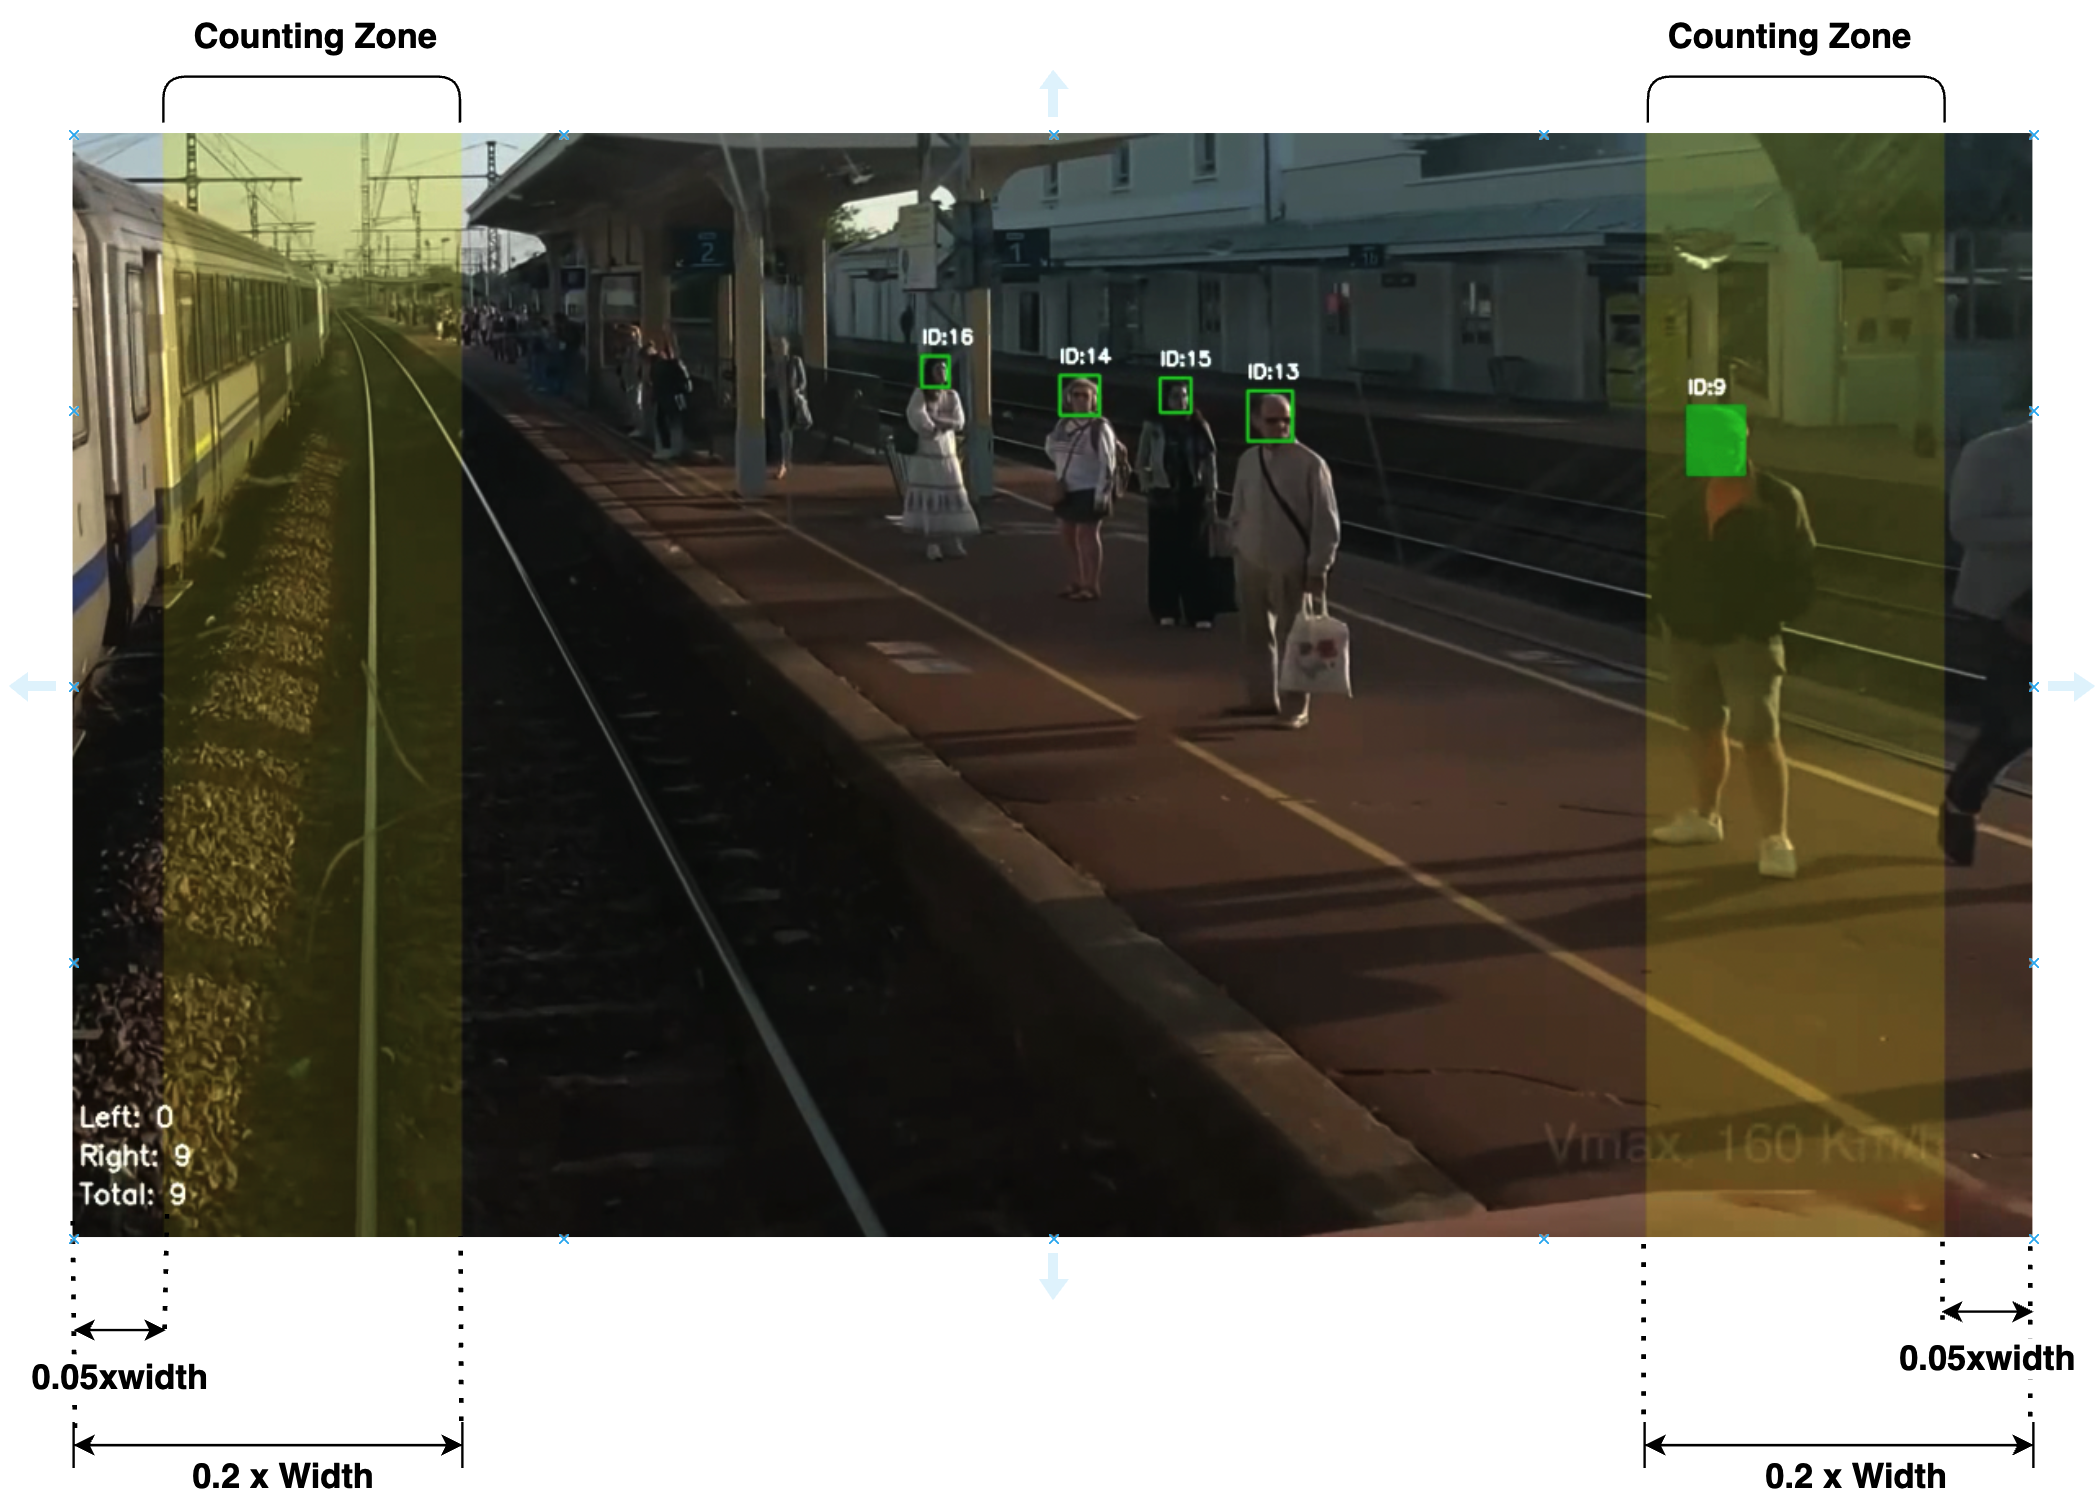
\includegraphics[width=0.49\textwidth]{pictures/VirtualCountingZone.png}
    \caption{Virtual Counting Band Illustration. The diagram shows the virtual counting zones positioned near the left and right image borders. The band is defined by start and end boundaries as proportions of image width (Start=0.05, End=0.20), creating a buffer region that tolerates brief occlusions and detection jitter. A target is counted only when it remains continuously within the band for a preset number of frames, providing robust counting under challenging conditions.}
    \label{fig:VirtualCountingZoneMethods}
\end{figure}

\textbf{Algorithm Implementation:}
\begin{enumerate}
    \item \textbf{Track State Management:} For each confirmed track, maintain state variables: consecutive\_in\_band\_frames, counted\_flag, and side\_assignment (left/right).
    \item \textbf{Band Membership Test:} Compute bounding box center $(u,v)$ and test if $u \in [\text{Start} \cdot W, \text{End} \cdot W]$ for left band or $u \in [W - \text{End} \cdot W, W - \text{Start} \cdot W]$ for right band.
    \item \textbf{Persistence Logic:} If track is in band, increment consecutive\_in\_band\_frames; otherwise reset to 0. When consecutive\_in\_band\_frames $\geq N$ and counted\_flag=False, set counted\_flag=True and increment corresponding side counter.
    \item \textbf{Deduplication:} Maintain global set of counted\_IDs to prevent double-counting across frames.
    \item \textbf{End-of-Video Compensation:} For tracks with consecutive\_in\_band\_frames $> 0$ but $< N$ at video end, apply compensation rule: if consecutive\_in\_band\_frames $\geq N/2$, count the track.
    \item \textbf{Final Aggregation:} Report left count, right count, and final count = max(left\_count, right\_count) to avoid non-platform bias.
\end{enumerate}

\subsection{Evaluation Metrics}

We evaluate our system using standard MOT metrics and counting metrics. For multi-object tracking evaluation, we adopt the CLEAR-MOT protocol \cite{bernardin2008evaluating} with metrics including Multiple Object Tracking Accuracy (MOTA), Multiple Object Tracking Precision (MOTP), Identity F1 Score (IDF1), and Identity Switches (IDSW). For identity-based evaluation, we use Identity Precision (IDP), Identity Recall (IDR), and IDF1 as defined in \cite{ristani2016performance}. 

For counting performance assessment, we employ standard regression metrics: Mean Absolute Error (MAE), Root Mean Squared Error (RMSE), Mean Absolute Percentage Error (MAPE), and Mean Error (ME) to quantify the discrepancy between predicted and ground-truth counts across all test videos.

\subsection{Camera Calibration}

To support the Phys-5D model's geometric constraints and depth estimation requirements, we perform camera calibration for each video sequence using fSpy software. Given the diverse camera setups and potential lens distortions across our dataset, we obtain multiple calibration results corresponding to different camera configurations. Based on the geometric constraint requirements in Equation~\ref{eq:geometric_constraints}, we calibrate the focal length $f$ and principal point coordinates $(c_u, c_v)$ for each video sequence. Our calibration results reveal three distinct camera configurations: (1) standard resolution cameras with focal length $f=1173.03$ pixels, (2) 4K cameras with $f=1600.3$ pixels, and (3) 2K cameras with $f=795.0$ pixels. These intrinsic parameters are essential for the Phys-5D model's 3D-to-2D projection constraints and accurate depth estimation.
